\documentclass[noamsthm]{beamercours}

\captionsetup[table]{font=small}

\begin{document}
\begin{frame}
        \reporttitleframe%
        {}
        {\centering %
                {\Large\sc Sur\, la\, Stabilité\, Interlangue\, des\, Catégories\, Morphosyntaxiques\par}
                \vspace{5pt}
                {Rapport de Stage de L3\par}
                \vspace{5pt}
                {Matthieu \textsc{Boyer}\par}
        }
        {../logo_lattice.png}
        {\centering %
                \vspace{3pt}
                {\sc Laboratoire\, Lattice \par}
                \vspace{4pt} %
                {\sc CNRS --- ENS-PSL --- Université Sorbonne Nouvelle\par}
                \vspace{6pt} %
                {Sous la direction de Mathieu \textsc{Dehouck}\par}}
\end{frame}

\section{Introduction}\label{sec:introduction}
\begin{frame}
        \frametitle{Contextualisation}\label{subsec:contextualisation}
        \begin{quote}
                There is a fundamental distinction between language-particular categories of languages (which descriptive linguists must describe by descriptive categories of their descriptions) and comparative concepts (which comparative linguists may use to compare languages).
                {\flushright \textit{Martin Haspelmath} \cite{Has18}}
        \end{quote}
\end{frame}

\begin{frame}
        \frametitle{Données et \textsc{Universal Dependencies}}\label{subsec:données}
        \begin{figure}
                \centering
                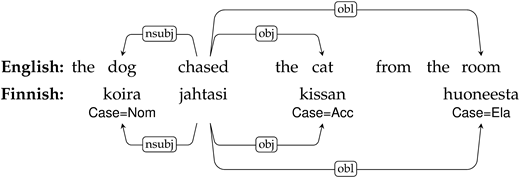
\includegraphics[width=\textwidth]{Figures/Visualisations/simplified_ud_annotation}
                \caption{Représentation d'une Phrase en Anglais et en Finnois et de ses Relations de Dépendances, source:\cite{UDv2}, \cite{UD214}}
                \label{fig:ud_annot}
        \end{figure}
\end{frame}

\section{Approche Géométrique}\label{sec:géométrie}
\begin{frame}
        \frametitle{Méthode Géométrique}
        On pose:
        \begin{itemize}
                \item $\R^{\abs{R}}$ où $R = \left\{\textit{reldep}\right\}$
                \item $\mathcal{T}$ l'ensemble des corpus et $\mathscr{C}$ l'ensemble des cas présents dans au moins un corpus
                \item $\nu(T, C)$ la représentation du cas $C$ dans le corpus $T$
                \item $\mE(C) = \left\{T \middle| \nu(T, C) \neq 0\right\}$
                \item $\cont(T) = \left\{C \middle| \nu(T, C) \neq 0\right\}$
        \end{itemize}
\end{frame}

\begin{frame}
        \frametitle{Avec la distance Cosinus}\label{subsec:cosinus}
        \only<1>{Pour:
                \begin{equation*}
                        d_{\cos}(v_{1},v_{2}) = \frac{\scalar{v_{1}\mid v_{2}}}{\norm{v_{1}}\norm{v_{2}}}
                \end{equation*}
                On calcule:
                \begin{equation*}
                        d_{\cos}\left(\nu\left(T_{1}, C_{1}\right), \nu\left(T_{2}, C_{2}\right)\right) \text{ où } T_{1}, T_{2} \in \mE(C_{1})\times \mE(C_{2})
                \end{equation*}}
        \only<2>{
                \renewcommand{\arraystretch}{1.1}
                \begin{table}
                        \centering
                        \resizebox{.9\textwidth}{!}{\begin{NiceTabular}{ccccccccc}
                                Cas & Abl & Acc & Dat & Gen & Ins & Loc & Nom & Voc \\
                                Premier Quartile & 0.037 & 0.020 & 0.022 & 0.032 & 0.056 & 0.027 & 0.026 & 0.000 \\
                                Médiane & 0.198 & 0.123 & 0.134 & 0.317 & 0.249 & 0.188 & 0.104 & 0.006 \\
                                Troisième Quartile & 0.416 & 0.302 & 0.341 & 0.823 & 0.449 & 0.400 & 0.225 & 0.047 \\
                                Moyenne & 0.259 & 0.196 & 0.214 & 0.421 & 0.282 & 0.243 & 0.159 & 0.058 \\
                        \CodeAfter
                                \begin{tikzpicture}
                                        \foreach \i in {1,...,6}
                                                {\draw[draw=vulm] (1|-\i) -- (10|-\i);}
                                        \draw[draw=vulm] (2|-1)--(2|-6);\end{tikzpicture}
                        \end{NiceTabular}}
                        \captionof{table}{Proximité Angulaire pour le \textit{Génitif}}
                        \label{tab:angle_gen}
                        \vspace{-3pt}
                        \centering
                        \resizebox{.9\textwidth}{!}{\begin{NiceTabular}{ccccccccc}
                                Cas& Abl & Acc & Dat & Gen & Ins & Loc & Nom & Voc \\
                                Premier Quartile & 0.020 & 0.038 & 0.018 & 0.026 & 0.035 & 0.020 & 0.620 & 0.003 \\
                                Médiane & 0.067 & 0.137 & 0.072 & 0.104 & 0.113 & 0.078 & 0.815 & 0.026 \\
                                Troisième Quartile & 0.158 & 0.272 & 0.161 & 0.225 & 0.211 & 0.156 & 0.912 & 0.075 \\
                                Moyenne & 0.115 & 0.188 & 0.119 & 0.159 & 0.153 & 0.115 & 0.739 & 0.072 \\
                        \CodeAfter
                                \begin{tikzpicture}
                                        \foreach \i in {1,...,6}
                                                {\draw[draw=vulm] (1|-\i) -- (10|-\i);}
                                        \draw[draw=vulm] (2|-1)--(2|-6);\end{tikzpicture}
                        \end{NiceTabular}}
                        \captionof{table}{Proximité Angulaire pour le \textit{Nominatif}}
                        \label{tab:angle_nom}
                \end{table}
        }
\end{frame}

\begin{frame}
        \frametitle{Système de Cas}
        On définit le Système de Cas d'une langue: $\mS(T) = \vect{\left(\nu(C, T)\right)_{C \in \cont(T)}}$
		\begin{itemize}
			\item Avec l'algorithme de Zassenhaus, on calcule:
			\begin{equation*}
				\left\{\dim(\mS(T_{1}) \cap \mS(T_{2}))\mid \left(T_{1}, T_{2}\right)\in \mT^{2}\right\}
			\end{equation*}
			\begin{equation*}
				\left\{\dim(\mS(T_{1}) + \mS(T_{2}))\mid \left(T_{1}, T_{2}\right) \in \mT^{2}\right\}
			\end{equation*}
			\item<2-> Avec la distance cosinus, on calcule:
			\begin{equation*}
				\left\{d_{\cos}(\nu(T_{1}, C_{1}), p_{\mS(T_{2})}(\nu(T_{1}, C_{1})))\mid T_{1}, T_{2} \in \mT^{2}, C_{1} \in \cont(T_{1})\right\}
			\end{equation*}
		\end{itemize}

\end{frame}

\begin{frame}
\frametitle{Distance Euclidienne}\label{subsec:l2}

On calcule alors, pour $C_{1}, C_{2}$ deux cas donnés,
\begin{equation*}
	\left\{d\left(\nu\left(T_{1}, C_{1}\right), \nu\left(T_{2}, C_{2}\right)\right)\mid T_{1}, T_{2} \in \mE(C_{1})\times \mE(C_{2})\right\}
\end{equation*}

\renewcommand{\arraystretch}{1.1}
\begin{table}
        \centering
        \resizebox{.9\textwidth}{!}{\begin{NiceTabular}{ccccccccc}
                Cas & Abl & Acc & Dat & Gen & Ins & Loc & Nom & Voc \\
                Premier Quartile & 0.605 & 0.315 & 0.552 & 0.521 & 0.535 & 0.595 & 0.569 & 0.842 \\
                Médiane & 0.781 & 0.476 & 0.725 & 0.715 & 0.695 & 0.764 & 0.722 & 0.992 \\
                Troisième Quartile & 1.002 & 0.695 & 0.950 & 0.936 & 0.929 & 0.993 & 0.965 & 1.115 \\
                Moyenne & 0.802 & 0.526 & 0.751 & 0.733 & 0.732 & 0.790 & 0.760 & 0.982 \\
        \CodeAfter
                \begin{tikzpicture}
                        \foreach \i in {1,...,6}
                                {\draw[draw=vulm] (1|-\i) -- (10|-\i);}
                        \draw[draw=vulm] (2|-1)--(2|-6);\end{tikzpicture}
        \end{NiceTabular}}
        \caption{Proximité pour la distance euclidienne avec l'\textit{Accusatif}}
	\label{tab_dist_acc}
\end{table}
\end{frame}

\begin{frame}
	\frametitle{Graphes des Voisins}
	\begin{figure}
		\centering
		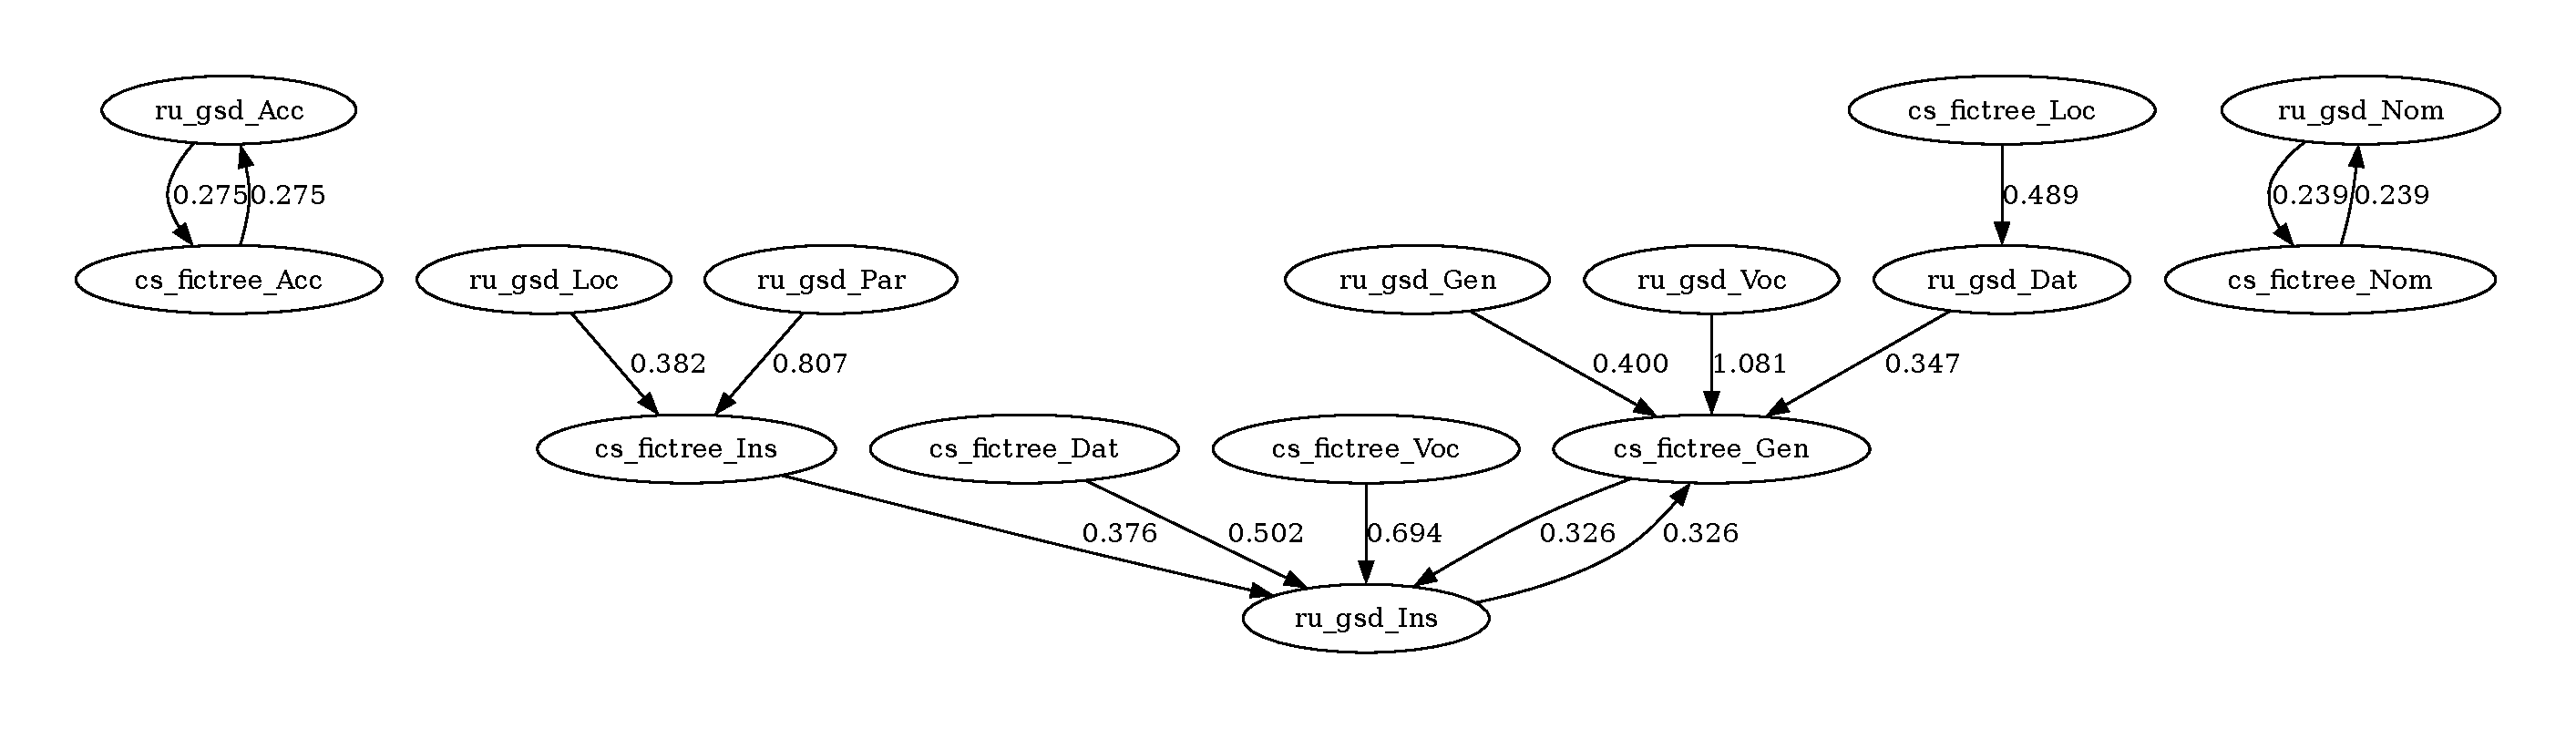
\includegraphics[width=\textwidth, height=.3\paperheight]{Figures/GNN/gnn_ru_gsd_cs_fictree}
		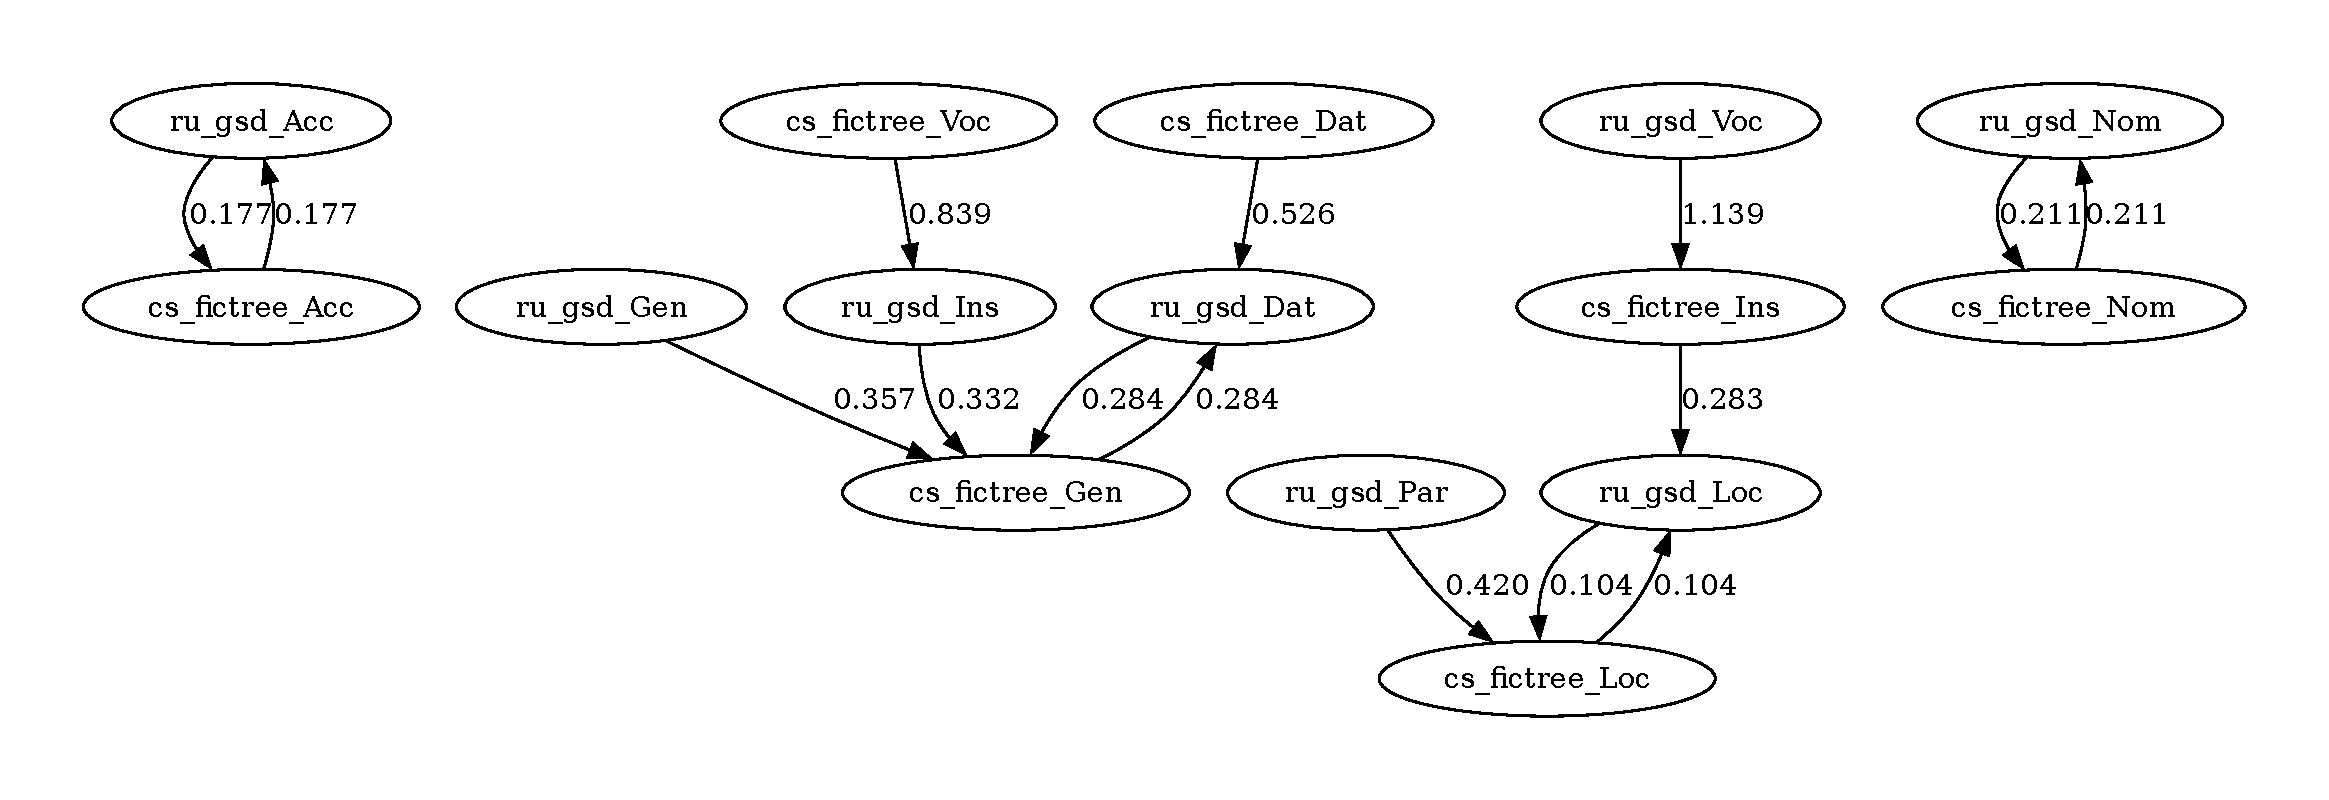
\includegraphics[width=\textwidth, height=.3\paperheight]{Figures/GNN/gnn_ru_gsd_cs_fictree_Nouns_Only}
		\caption{Graphes des Plus Proches Voisins Russe-Tchèque}
		\label{fig_gnn_nouns_ru_cz}
	\end{figure}
\end{frame}

% TODO: Ajouter des trucs

\section{Visualisation des Données}\label{subsec:vis}

\begin{frame}
\frametitle{PCA}\label{subsub:pca}
\begin{figure}
	\begin{minipage}{.45\textwidth}
	\begin{center}
	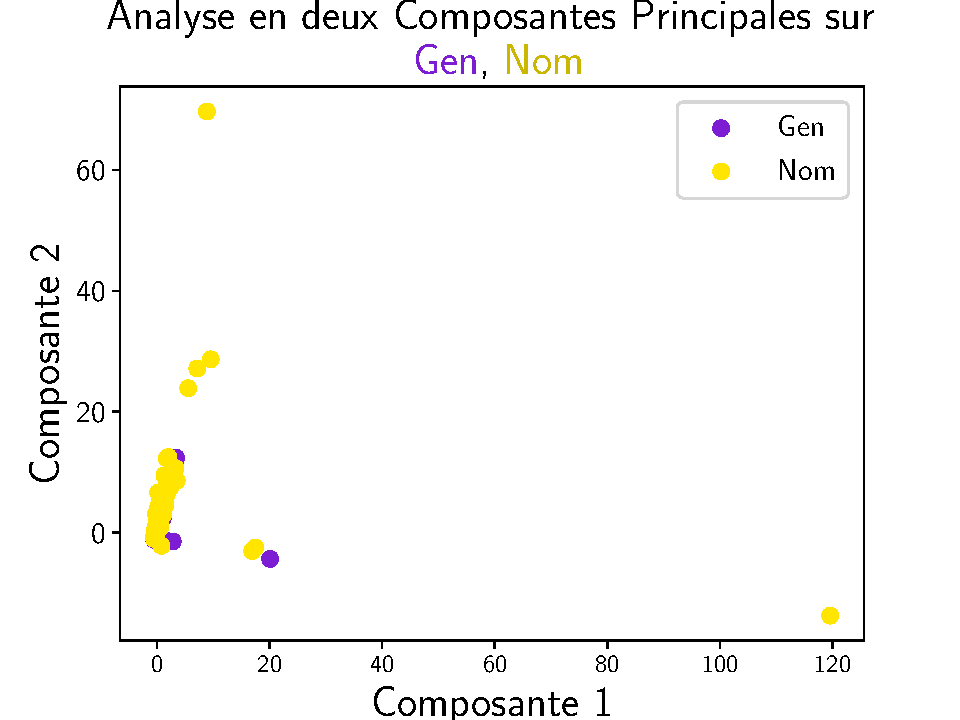
\includegraphics[width=\linewidth]{Figures/Visualisations/pca_Gen_Nom}
	\end{center}
	\end{minipage}
	\begin{minipage}{.45\textwidth}
	\begin{center}
	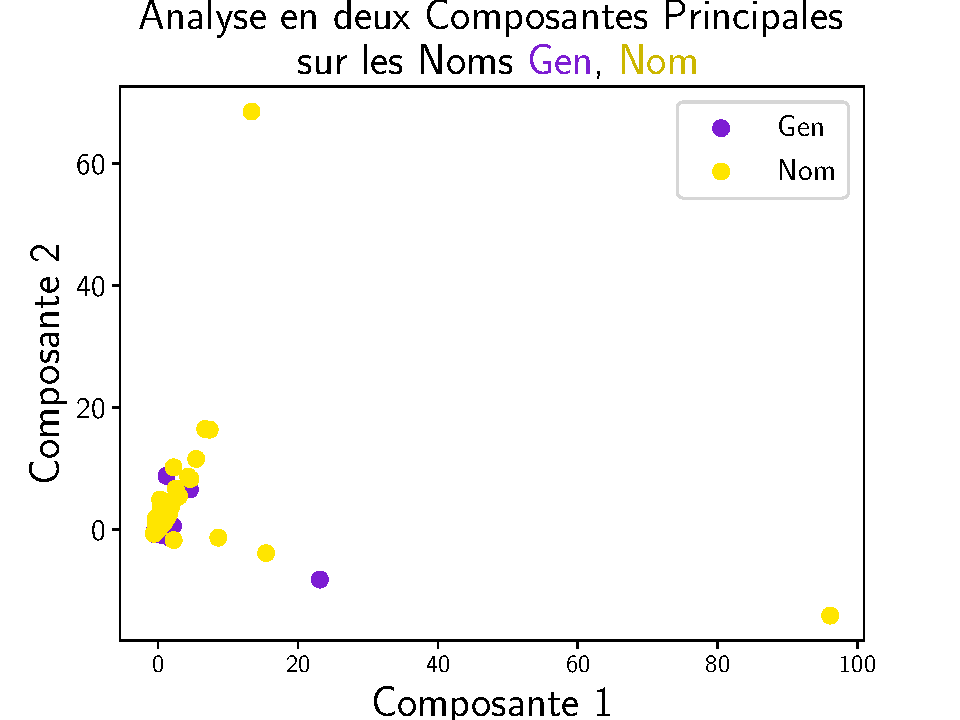
\includegraphics[width=\linewidth]{Figures/Visualisations/pca_Gen_Nom_Nouns}
	\end{center}
	\end{minipage}
	\caption{Représentations de l'Analyse en deux Composantes Principales sur le Génitif et le Nominatif}
	\label{fig:pca}
\end{figure}
\end{frame}


\begin{frame}
\frametitle{Analyse Topologique des Données -- 1}\label{subsub:tda}

\begin{figure}
\begin{minipage}{.45\textwidth}
	\begin{center}
	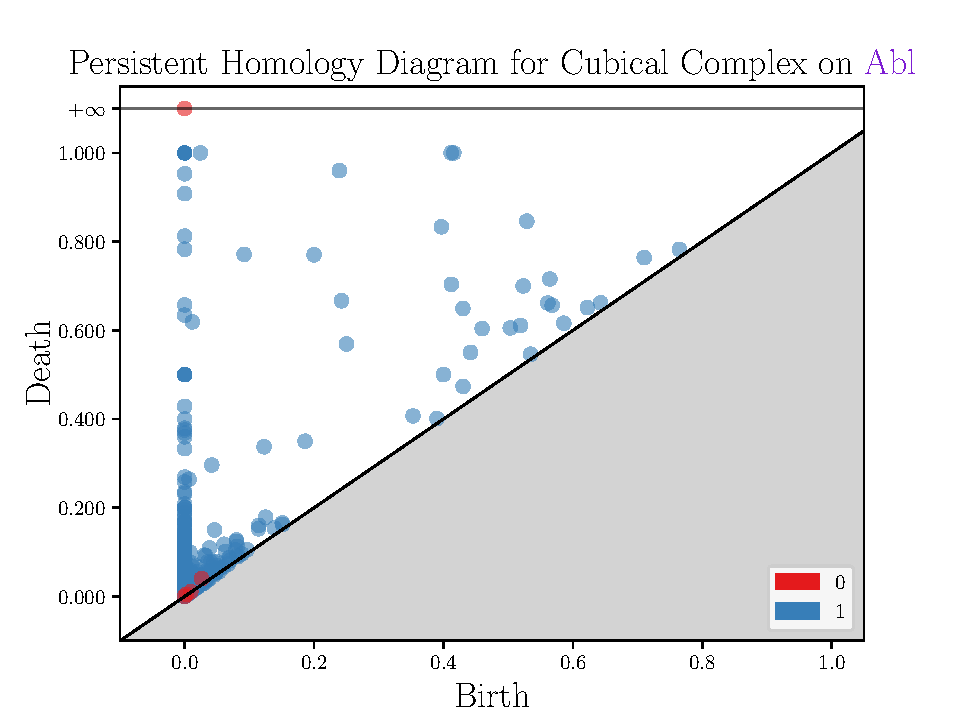
\includegraphics[width=\linewidth]{Figures/Visualisations/cc_Abl}
	\end{center}
\end{minipage}
\begin{minipage}{.45\textwidth}
	\begin{center}
	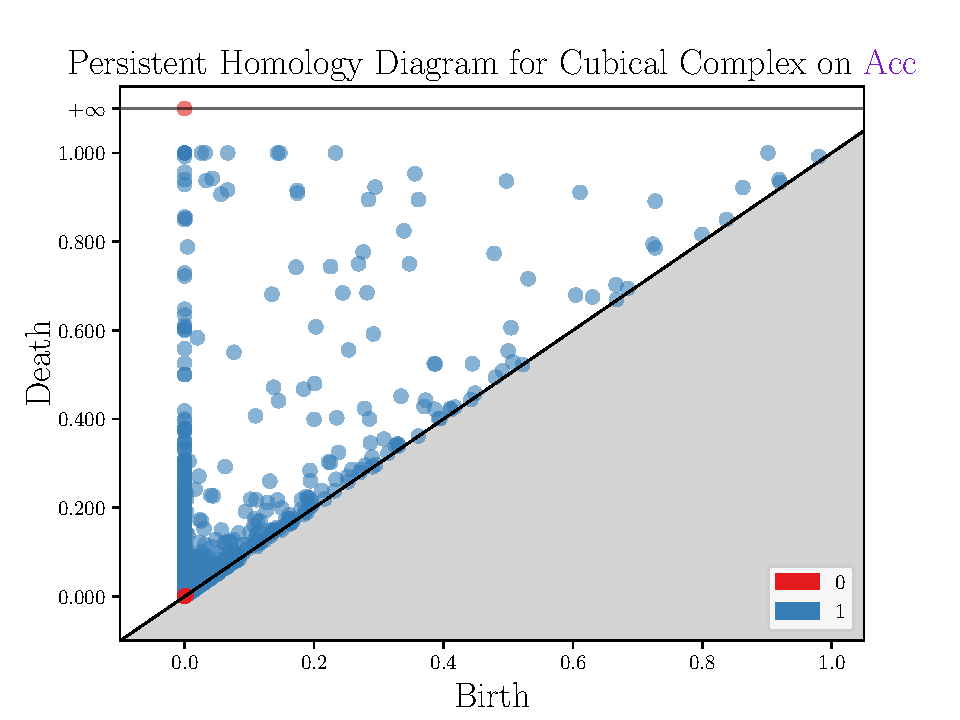
\includegraphics[width=\linewidth]{Figures/Visualisations/cc_Acc}
	\end{center}
\end{minipage}
\caption{Représentations de l'Homologie Persistente du Complexe Cubique sur $\{\tt Abl,Acc\}$}
\label{fig_cc_hom}
\end{figure}
\end{frame}

\begin{frame}
	\frametitle{Analyse Topologique des Données -- 2}
	\only<1>{La distance-$p$ de Wasserstein pour $p \in \left[1, +\infty\right]$ entre deux mesures de probabilités $\mu, \pi$ dont les moments d'ordre $p$ sont finis est:
		\begin{equation*}
		W_{p}(\mu, \pi) = \inf_{\gamma\in\Gamma\left(\mu, \pi\right)}\sqrt[p]{\mathbb{E}_{(x, y) \sim \gamma}d(x, y)^{p}}
		\end{equation*}
		où $\Gamma\left(\mu, \pi\right)$ est l'ensemble des couplages de $\mu, \pi$.
	}

	\only<2>{%
		\begin{table}
		\centering
		\begin{tabular}{c|ccccc}
			\toprule
			Cas & Abl & Acc & Dat & Loc & Gen\\
			\midrule
			Abl & 0.00 & 2.45 & 3.11 & 1.94 & 3.85\\
			Acc & 2.45 & 0.00 & 1.33 & 1.25 & 1.79\\
			Dat & 3.11 & 1.33 & 0.00 & 1.63 & 1.27\\
			Loc & 1.94 & 1.25 & 1.63 & 0.00 & 2.26\\
			Gen & 3.85 & 1.79 & 1.27 & 2.26 & 0.00\\
			\bottomrule
		\end{tabular}
		\caption{Distances de Wasserstein entre les Diagrammes de Persistence des Complexes Cubiques pour quelques Cas}
		\label{tab_wass_cc}
		\end{table}
	}
\end{frame}

\begin{frame}
	\frametitle{Analyse Topologique des Données -- 3}
	\only<1>{
	\begin{figure}
	\begin{minipage}{.45\textwidth}
		\begin{center}
		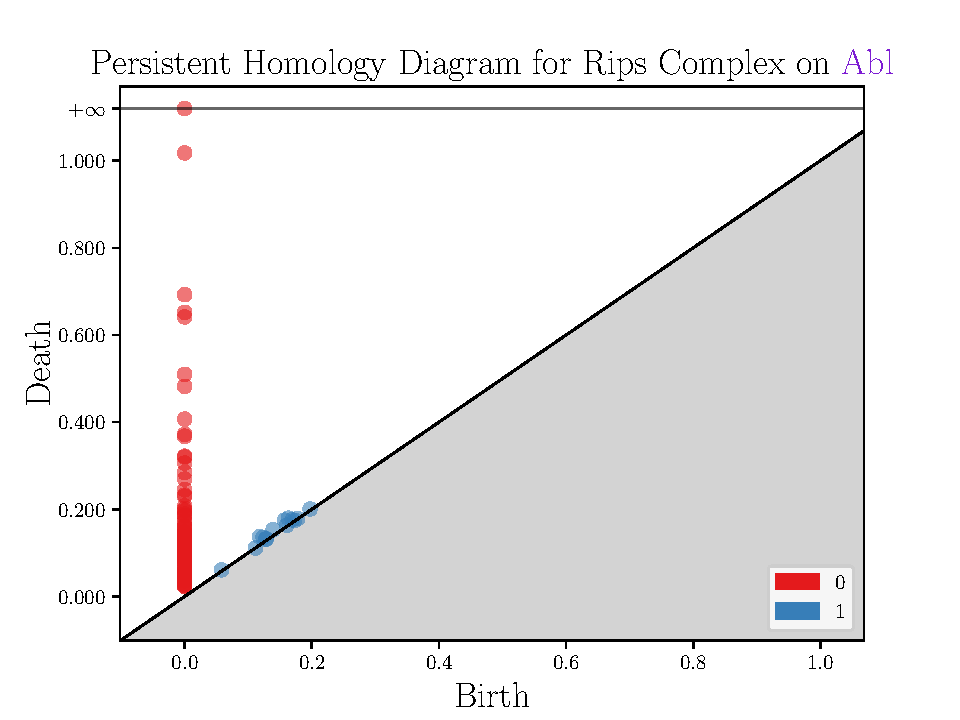
\includegraphics[width=\linewidth]{Figures/Visualisations/rc_Abl.pdf}
		\end{center}
	\end{minipage}
	\begin{minipage}{.45\textwidth}
		\begin{center}
		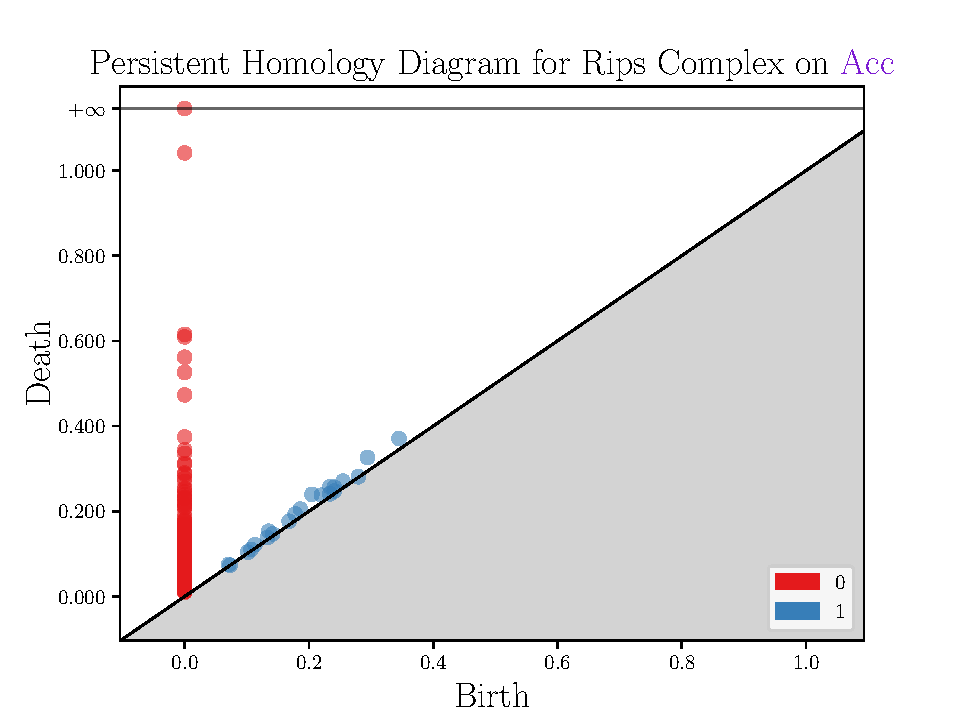
\includegraphics[width=\linewidth]{Figures/Visualisations/rc_Acc.pdf}
		\end{center}
	\end{minipage}
	\caption{Représentations de l'Homologie Persistente du Complexe de Rips sur $\{\tt Abl,Acc\}$}
	\label{fig_rc_hom}
	\end{figure}
	}
	\only<2>{
	\begin{table}
		\centering
		\begin{tabular}{c|cccccc}
			\toprule
			Cas & Abl & Acc & Dat & Gen & Loc & Nom\\
			\midrule
			Abl & 0.00 & 0.89 & 1.27 & 0.82 & 1.09 & 0.94\\
			Acc & 0.89 & 0.00 & 1.01 & 0.42 & 1.03 & 0.91\\
			Dat & 1.27 & 1.01 & 0.00 & 0.87 & 1.47 & 0.76\\
			Gen & 0.82 & 0.42 & 0.87 & 0.00 & 0.84 & 0.87\\
			Loc & 1.09 & 1.03 & 1.47 & 0.84 & 0.00 & 1.48\\
			Nom & 0.94 & 0.91 & 0.76 & 0.87 & 1.48 & 0.00\\
			\bottomrule
		\end{tabular}
		\caption{Distances de Wasserstein entre les Diagrammes de Persistence des Complexes de Rips pour quelques Cas}
		\label{tab_wass_rc}
		\end{table}}
\end{frame}

\begin{frame}
	\frametitle{t-SNE}\label{subsub:tsne}
	% L'algorithme définit une distribution $D_{1}$ de probabilités sur les paires de points de l'espace de départ (si $x, y$ sont proches alors $D_{1}(x \mid y)$ est proche de $1$) et construit alors une distribution $D_{2}$ sur les paires de points d'un espace à $2$ dimensions minimisant la divergence de Kullback-Leibler $\sum_{x, y}D_{1}(x \mid y)\log\frac{D_{1}(x\mid y)}{D_{2}(x\mid y)}$ entre $D_{1}$ et $D_{2}$.
	% \cite{tSNE}.
	\begin{figure}
	\begin{minipage}{.45\textwidth}
		\begin{center}
			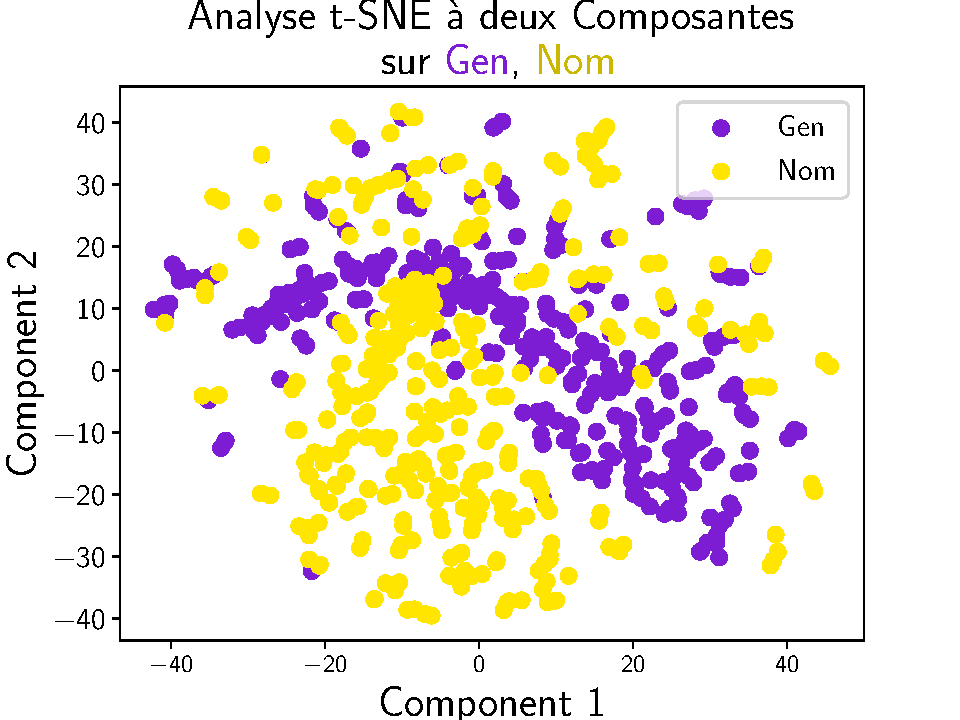
\includegraphics[width=\linewidth]{Figures/Visualisations/tsne_Gen_Nom.pdf}
		\end{center}
	\end{minipage}
	\begin{minipage}{.45\textwidth}
		\begin{center}
			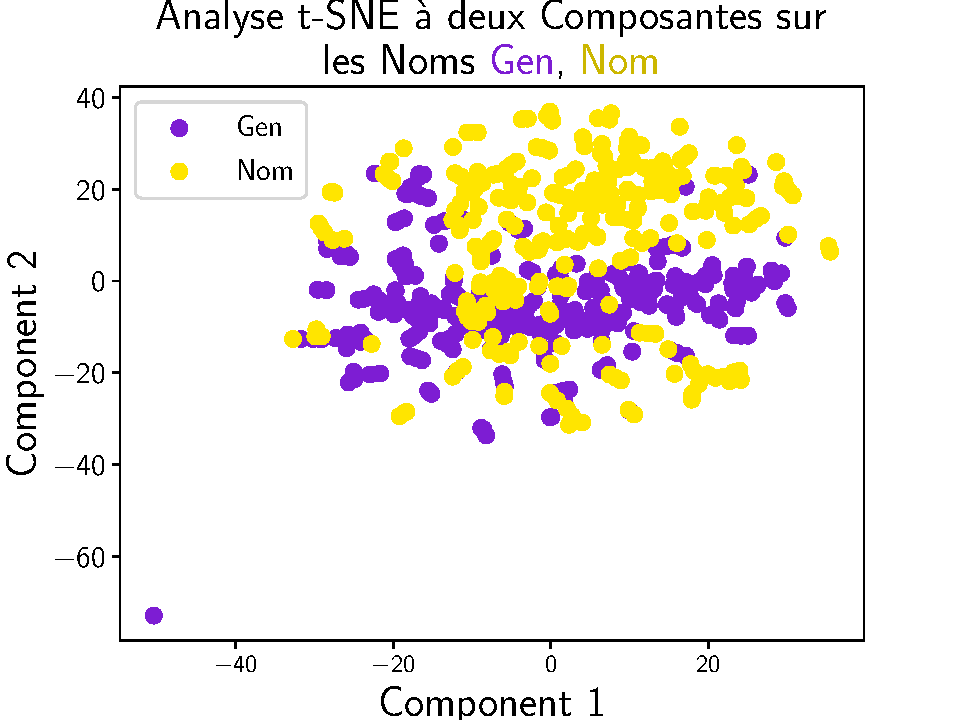
\includegraphics[width=\linewidth]{Figures/Visualisations/tsne_Gen_Nom_Nouns.pdf}
		\end{center}
	\end{minipage}
	\caption{Représentations de l'Analyse t-SNE (cf. \cite{tSNE}) à deux Composantes sur le Génitif et le Nominatif}
	\label{fig_tsne}
	\end{figure}
\end{frame}


\begin{frame}
\frametitle{Clustering avec ToMATo}\label{subsub:tomato}
%On applique l'algorithme présenté dans \cite{ToMATo} avec la bibliothèque \texttt{Gudhi} (\cite{Gudhi}) sur des paires de cas, pour essayer de construire des clusters.
Cet algorithme utilise les ensembles de sur-niveau associés à une fonction $f$ (les $F^{\alpha} = f^{-1}\left(\left[\alpha, +\infty\right[\right)$) pour construire le diagramme de persistence (voir \cite{tldrtda} et \cite{ToMATo}).

\begin{figure}
\begin{minipage}{.45\textwidth}
	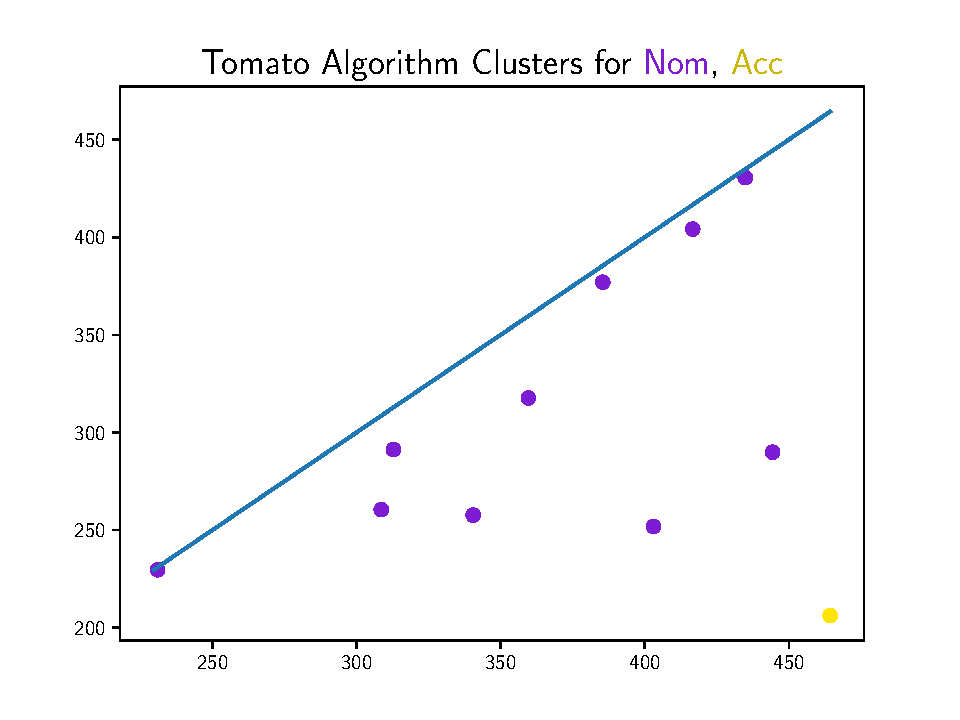
\includegraphics[width=\linewidth]{Figures/Visualisations/tomato_Nom_Acc_Nouns}
\end{minipage}
\begin{minipage}{.45\textwidth}
	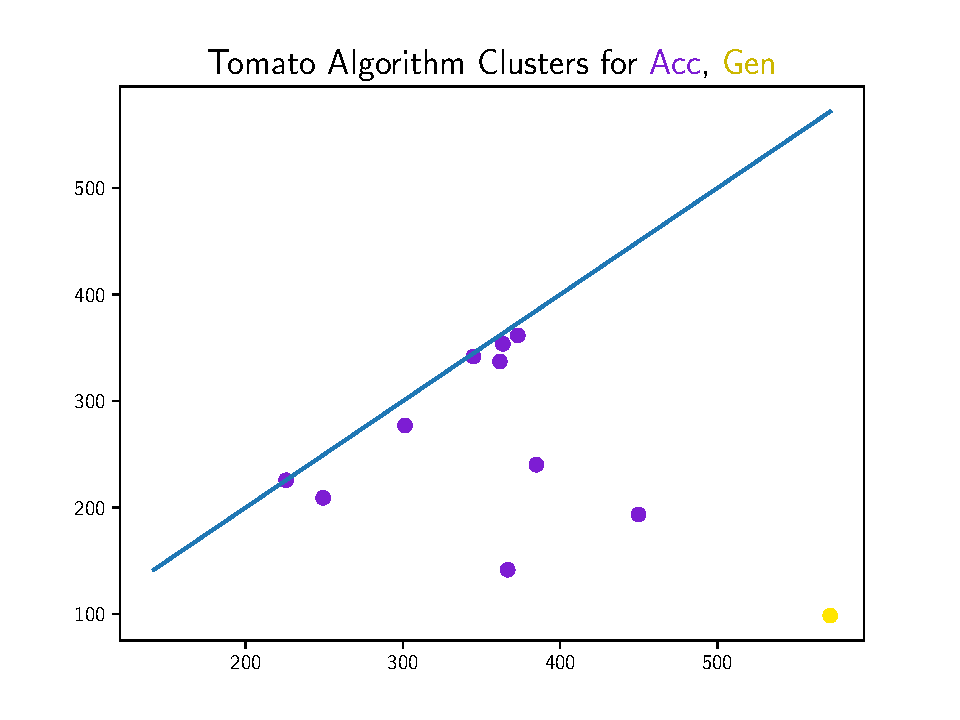
\includegraphics[width=\linewidth]{Figures/Visualisations/tomato_Acc_Gen_Nouns}
\end{minipage}
\caption{Représentations des Clusters trouvés par l'Algorithme ToMATo sur les Paires de $\{\tt Acc,Nom,Gen\}$}
\label{fig_tomato}
\end{figure}
\end{frame}

\begin{frame}
\frametitle{Clustering avec KNN}\label{subsub:knn}
\begin{table}
	\centering
	\pgfplotsset{colormap/jet}
\pgfplotstabletypeset[
	color cells={min=0, max=250},
	col sep=comma,
	row sep=crcr,
]{
	Acc,Gen,Loc,Nom\\
	130,62,51,34\\
	69,156,16,42\\
	35,57,29,34\\
	29,28,9,227\\
}
	\caption{Heatmap de l'Algorithme KNN avec $k = 11$ sur \texttt{Acc, Gen, Loc, Nom}}
	\label{tab_knn}
\end{table}
\end{frame}

\section{Approche Probabiliste}\label{sec:probas}
\begin{frame}
\frametitle{Barycentrisation -- Théorie}\label{subsec:bary}
\begin{description}
		\item[Nom] Agent (sujet) d'un verbe
		\item[Acc] Patient (objet direct) d'un verbe
		\item[Erg] Agent (et donc patient) d'un verbe intransitif (sans objet), ou patient d'un verbe transitif
		\item[Abs] Agent d'un verbe transitif
		\item[Gen] Complément du nom
		\item[Dat] Objet indirect d'un verbe
	\end{description}

\end{frame}

\begin{frame}
\frametitle{Barycentrisation -- Empirique}
\only<1>{
On associe à un cas une variable aléatoire $\mathcal{R}(C)$.
On peut alors calculer $\E(\mathcal{R}(C))$ mais également le barycentre de ses réalisations pour la distance-$1$ de Wasserstein.
On rappelle par ailleurs que le barycentre de $n$ points pour une distance $d$ est le point $P$ qui minimise l'énergie $E$ associée:

\begin{equation*}
	P = \arg\min_{x} E\left(x, \left(x_{i}\right)_{i \in \onen{n}}\right) \text{ avec } E\left(x, \left(x_{i}\right)_{i \in \onen{n}}\right) = \frac{1}{n}\sum_{i = 1}^{n} d(x, x_{i})
\end{equation*}
}
\only<2>{%
\begin{table}
\centering
\renewcommand{\arraystretch}{1.3}
\begin{NiceTabular}{llccccc}
				\bf Cas & \bf Prototype &\tt iobj & \tt nmod & \tt nsubj & \tt obj & \tt obl\\

	\multirow[c]{2}{*}{\bf\sc Nom}  & Uniforme    & 0.001 & 0.080 & 0.556 & 0.074 & 0.050\\
									& Wasserstein & 0.000 & 0.049 & 0.654 & 0.093 & 0.038\\

	\multirow[c]{2}{*}{\bf\sc Acc}  & Uniforme    & 0.006 & 0.078 & 0.038 & 0.625 & 0.205\\
									& Wasserstein & 0.000 & 0.072 & 0.019 & 0.576 & 0.259\\

	\multirow[c]{2}{*}{\bf\sc Gen}  & Uniforme    & 0.009 & 0.674 & 0.039 & 0.056 & 0.149\\
									& Wasserstein & 0.000 & 0.729 & 0.031 & 0.045 & 0.179\\

	\CodeAfter
	\begin{tikzpicture}
		\foreach \i in {2, 4, 6} {\draw[black] (1|-\i) -- (8|-\i);}
		\draw[black] (2|-1) -- (2|-8);
	\end{tikzpicture}
\end{NiceTabular}
\caption{Représentation des Principales \textit{reldep} des Prototypes pour quelques Cas sur les Noms}
\label{tab_proto}
\end{table}}
\end{frame}


\begin{frame}
	\frametitle{Comparaison aux Données}
	\begin{figure}
\centering
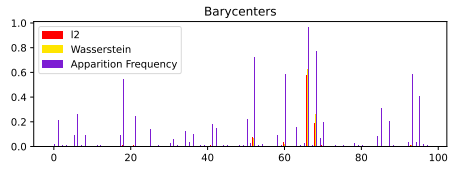
\includegraphics[width=\linewidth]{Figures/Visualisations/Nouns_Wasserstein_Barycenter_Acc_Barys}
\caption{Représentation des Données et des Prototypes proposés pour les Noms à l'Accusatif}
\label{fig_proto}
\end{figure}
\end{frame}


\begin{frame}
\frametitle{Représentation des adpositions dans UD}\label{subsec:adpos}
\begin{table}
	\centering
	\renewcommand{\arraystretch}{1.3}
	\begin{NiceTabular}{>{\sc}rcccccc}
		\bf Adposition & \tt advcl &\tt iobj & \tt nmod & \tt obj & \tt obl\\
		À    & 0.01668 &  & 0.17343 & 0.00381 & 0.63373\\

		Pour & 0.29543 & & 0.15867   & 0.00024 & 0.41168\\
		En   & 0.08128 &  & 0.17115  & 0.00358 & 0.54076\\
		Vers & 0.00262 &  & 0.35741  & & 0.62160\\

		De   & 0.02096 &  & 0.67966  & 0.01312 & 0.14296\\
		Sous & 0.00217 & & 0.22898 & 0.72797 & \\
		Sauf & 0.10714 & & 0.22619 & & 0.38095\\
	\CodeAfter
	\begin{tikzpicture}
		\foreach \i in {2,...,9} {\draw[black] (1|-\i) --  (8|-\i);}
	\end{tikzpicture}
	\end{NiceTabular}
	\caption{Quelques adpositions françaises, suivant \cite{morphenglish}}
	\label{tab:adpos_fr}
\end{table}

\end{frame}

\section{Conclusion}

\begin{frame}
	\frametitle{Conclusion}
	Nous avons trouvé:
	\begin{itemize}
		\item Une structure géométrique générale de la syntaxe des cas
		\item Des classes d'équivalence syntaxique de cas
		\item Des disparités dans les manières d'annoter les cas
		\item Des preuves appuyant la thèse de Martin \textsc{Haspelmath}
		\item Une manière d'annoter des adpositions
	\end{itemize}
	Il reste à étudier:
	\begin{itemize}
		\item la viabilité d'un parser syntaxique basé sur des fusions de cas;
		\item l'applicabilité d'un parser d'une langue sur une autre langue proche en système de cas.
	\end{itemize}
\end{frame}

\begin{frame}[t, allowframebreaks]
	\frametitle{Bibliographie}
	\bibliographystyle{alpha-fr}
	\bibliography{report}
\end{frame}

\end{document}
